% 图 3.1 —— 手工重建（两个相交圆 E / E'，一个实心点 w，三个空心圈 x / y / x'）
%
% 参数全部来自 `checks/probe.py 3.1` 的**区域内精测**，不是估的：
%   · 两圆解析：e0 c=(261.6,123.4) r=106.1 ；e1 c=(119.7,127.6) r=106.3
%     —— 到墨迹距离的中位/90 分位都是 0.00，圆拟合无残差
%   · 线宽实测 4.0
%   · 字标：字号由「字形框高度」反推（probe ③ 直接给可粘贴的 \node 行）
%
% ⚠ 本文件是 `emit_hand.py` 出的**自动稿改了这两处**之后的样子
%   （自动稿见 git 历史 / 或跑 `emit_hand.py 3.1 --force` 重出）：
%   ① 三个点标记 probe 认成了小写字母 `o`，实际是**空心圈 ⊙**。
%      尺寸与实心点同级：外径 17.4（实心点 r=8.70），环厚 = 线宽 4.0
%      ⇒ `\draw ... circle (6.7)`（6.7 + 4.0/2 = 8.7）
%   ② `E'` 的**撇**被拆成两条：`E`(357.2,31.5) + `'`(373.0,22.2)。
%      合成一条 `\textit{E}'`，锚在两者合成中心 (360.0,30.5)。
\documentclass[12pt]{standalone}
\usepackage{fontspec}
\setsansfont{Arial}
\usepackage{tikz}
\begin{document}
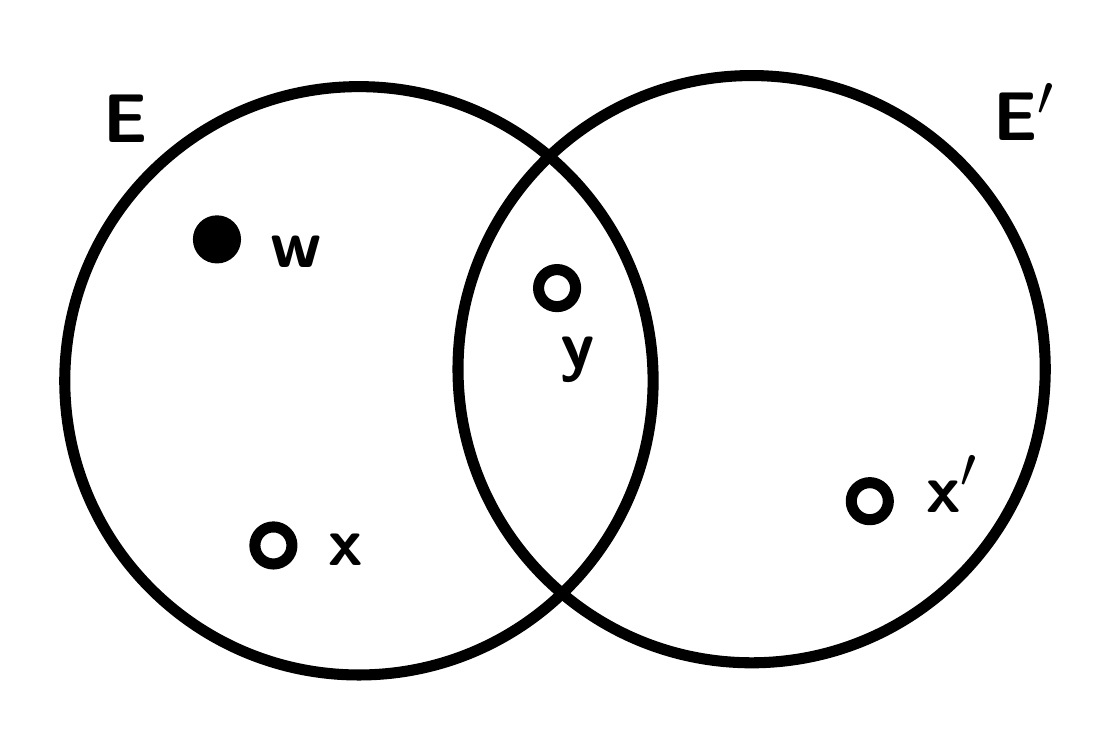
\begin{tikzpicture}[x=1pt, y=-1pt, line width=4.0pt, line cap=round, line join=round]

  % ════ 两个相交圆 ════
  \draw (261.6,123.4) circle (106.1);
  \draw (119.7,127.6) circle (106.3);

  % ════ 一个实心点（w）════
  \fill (68.4,76.5) circle (8.7);

  % ════ 三个空心圈（x / y / x'）════
  \draw (88.8,187.1) circle (6.7);
  \draw (191.3,94.1) circle (6.7);
  \draw (304.3,171.1) circle (6.7);

  % ════ 标签 ════
  % ⚠ 全部 fill=white：文字在最上层，否则和圆边界交叉干扰
  \node[anchor=center,inner sep=0pt,fill=white,font=\fontsize{29.6}{37.0}\selectfont] at (35.3,33.0) {\textsf{\textbf{\textit{E}}}};
  \node[anchor=center,inner sep=0pt,fill=white,font=\fontsize{29.6}{37.0}\selectfont] at (360.0,30.5) {\textsf{\textbf{\textit{E}$'$}}};
  \node[anchor=center,inner sep=0pt,fill=white,font=\fontsize{29.6}{37.0}\selectfont] at (97.2,80.8) {\textsf{\textbf{\textit{w}}}};
  \node[anchor=center,inner sep=0pt,fill=white,font=\fontsize{31.0}{38.7}\selectfont] at (115.0,188.6) {\textsf{\textbf{\textit{x}}}};
  \node[anchor=center,inner sep=0pt,fill=white,font=\fontsize{30.5}{38.1}\selectfont] at (198.8,119.8) {\textsf{\textbf{\textit{y}}}};
  \node[anchor=center,inner sep=0pt,fill=white,font=\fontsize{31.0}{38.7}\selectfont] at (334.0,165.0) {\textsf{\textbf{\textit{x}$'$}}};

  \path[use as bounding box] (0,0) rectangle (381,245);
\end{tikzpicture}
\end{document}
